\documentclass[11pt, spanish]{report}
\usepackage[spanish]{babel}
\usepackage{graphicx}
\selectlanguage{spanish}
\usepackage[utf8]{inputenc}
% Title Page
\title{Central Meteorológica con fines educativos}
\author{Raul Giucich}


\begin{document}
\maketitle

\begin{abstract}

Este trabajo tiene como objetivo construir una central meteorológica con elementos que en su gran mayoría se pueden conseguir en ferreterías y negocios de electrónica locales. Los sensores, MODEM y el PIC que los controla son los únicos elementos importados. Todo el software producido y utilizado durante este trabajo será Open Source.

El público objetivo de este producto es la educación escolar básica, tanto docentes como alumos a partir de los 12 años, y permitirá introdudir en la escuela la electrónica y la informática desde un enfoque de producción y no de consumo. El uso permitirá complementar las materias de matemática, medio natural, ciencias de la salud y el método científico. La construcción permitirá desarrollar el trabajo en equipo y habilidades relacionadas al trabajo técnico como la presición, la medición y el diagnóstico.

La central construida tendrá conexión a Internet y podrá enviar los datos a un sitio de soporte que contendrá la geolocalización de las centrales, y materiales educativos relacionados al clima y tratamiento de los datos.


\end{abstract}

\section{Descripción}
El trabajo de compone de 3 elementos:
\begin{enumerate}
\item Central propiamente dicha:
\begin{itemize}
\item Mediciones: Velocidad del viento, dirección del viento, temperatura, humedad relativa ambiente, cantidad de lluvia y calidad del aire (NO2 - Dióxido de Nitrógeno y CO2 ' Anhidrido carbónico).
\item Control: Arduino UNO o NANODE utilizando los puertos analógicos y digitales para la captura.
\item Conexiones: Conectores RJ11 de 4 hilos (V+, GND, DATA, AUX).
\item Montaje: Componentes soldados sobre tarjetas perforadas.
\item Fuente: Fuente de corriente 9v, 650mA.
\item Transmisión de datos: Ethernet Shield de Arduino o Puerto Ethernet de NANODE, Modem GSM.
\item Infraestructura: Pagoda para los sensores de temperatura, humedad y calidad del aire. El pluviómetro, velocidad y dirección del viento utilizando latas con estructura interna reforzada, caños de PVC para la elevación.
\item Software: utilizando Arduino Programming Language y SDK Arduino.
\item Normalización de datos: Utilizar open data con nivel de 4 estrellas de las 5 de 5stardata.info
\end{itemize}
\item Manual de como construir la central y conectarla a Internet.
\begin{itemize}
\item Lista de compra de materiales y herramientas a utilizar.
\item Esquemáticos de los circuitos.
\item Guía de soldado, verificación y montaje de componentes.
\item Guía de construcción y montaje de la infraestructura.
\item Registro de la central en la APP web y uso de la API para la publicación y consumo de los datos.
\end{itemize}
\item Aplicación WEB de soporte para almacenamiento de datos y publicación de los mismos.
\begin{itemize}
\item Registro de una central: Geolocalización y disponibilidad de sensores.
\item Agregación de datos capturados para cumplimiento de estrellas de Open Data
\item Visualización de datos capturados
\item Descarga en archivos y API de acceso a datos.
\item Material educativo de referencia para la utilización de los datos en el aula.
\item Software: Framework Laravel 4, Postgres, Postgis, AngularJS, ZURB Foundation. Publicado en yvytu.net
\end{itemize}
\end{enumerate}

\section{Alcance}
Inicia con la Investigación sobre como funciona una central meteorológica y la sistematización de datos de Open Data. 
Como productos entregables
\begin{enumerate}
\item Una central montada y en funcionamiento en el predio de un colegio en la ciudad de Lambaré
\item Aplicación WEB publicada en Internet.
\item Copia del manual publicada.
\end{enumerate}

\section{Esquema Gráfico}
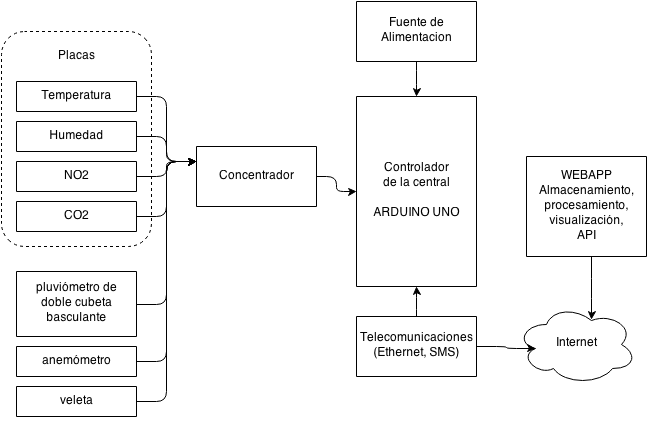
\includegraphics[width=0.9\textwidth,natwidth=648,natheight=421]{Central.png}



\end{document}          
